\documentclass[12pt]{article}

% pacchetti 
\usepackage[italian]{babel}
\usepackage{graphicx}
\usepackage{svg}

\usepackage{geometry}
 \geometry{
 a4paper,
 left=25mm,
 top=25mm,
 }
 
\usepackage{hyperref}
\hypersetup{
    colorlinks,
    citecolor=blue,
    filecolor=blue,
    linkcolor=blue,
    urlcolor=blue
}

%bibliography
\usepackage[sorting=none, isbn=false, eprint=false]{biblatex}
\addbibresource{bibliography.bib}


% set images path 
\graphicspath{ {./images/} }
% specify different fonts for headings 

\usepackage{color}

\definecolor{dkgreen}{rgb}{0,0.6,0}
\definecolor{mauve}{rgb}{0.58,0,0.82}
\definecolor{chromeyellow}{rgb}{1.0, 0.65, 0.0}

%______________Team's comments______________%

\newcommand{\edoardo}[1]{{\bf \color{red} Edoardo: #1 }}
\newcommand{\andrea}[1]{{\bf \color{mauve} Andrea: #1 }}
\newcommand{\davide}[1]{{\bf \color{chromeyellow} Davide: #1 }}
\newcommand{\piaget}[1]{{\bf \color{dkgreen} Piaget: #1 }}

%______________________Listing________________________%

\usepackage{listings}

\definecolor{codegreen}{rgb}{0,0.6,0}
\definecolor{codegray}{rgb}{0.5,0.5,0.5}
\definecolor{codepurple}{rgb}{0.58,0,0.82}
\definecolor{backcolour}{rgb}{0.95,0.95,0.92}

\lstdefinestyle{mystyle}{
    language=Java,
    aboveskip=5mm,
    belowskip=5mm,
    columns=flexible,
    backgroundcolor=\color{backcolour},   
    commentstyle=\color{codegreen},
    keywordstyle=\color{magenta},
    numberstyle=\tiny\color{codegray},
    stringstyle=\color{codepurple},
    basicstyle=\ttfamily\footnotesize,
    breakatwhitespace=false,         
    breaklines=true,                 
    captionpos=t,                    
    keepspaces=true,                 
    numbers=left,                    
    numbersep=5pt,                  
    showspaces=false,                
    showstringspaces=false,
    showtabs=false,                  
    tabsize=2
}

\lstset{style=mystyle}




\begin{document}
% pagina iniziale

\begin{figure}
    \centering
    
\includegraphics[width=0.2\linewidth]{images/unito_logo.jpg}
\end{figure}

\begin{center}
    \vspace{5ex}
    {\huge \textbf{Esame di Design Patterns}}
    \vspace{5ex}
\end{center}

\begin{center}
    Andrea Balbo Mossetti \\
    Davide Marietti \\
    Piaget Bouka \\
    Edoardo Pastori
\end{center}

\vspace{10ex}

\begin{center}

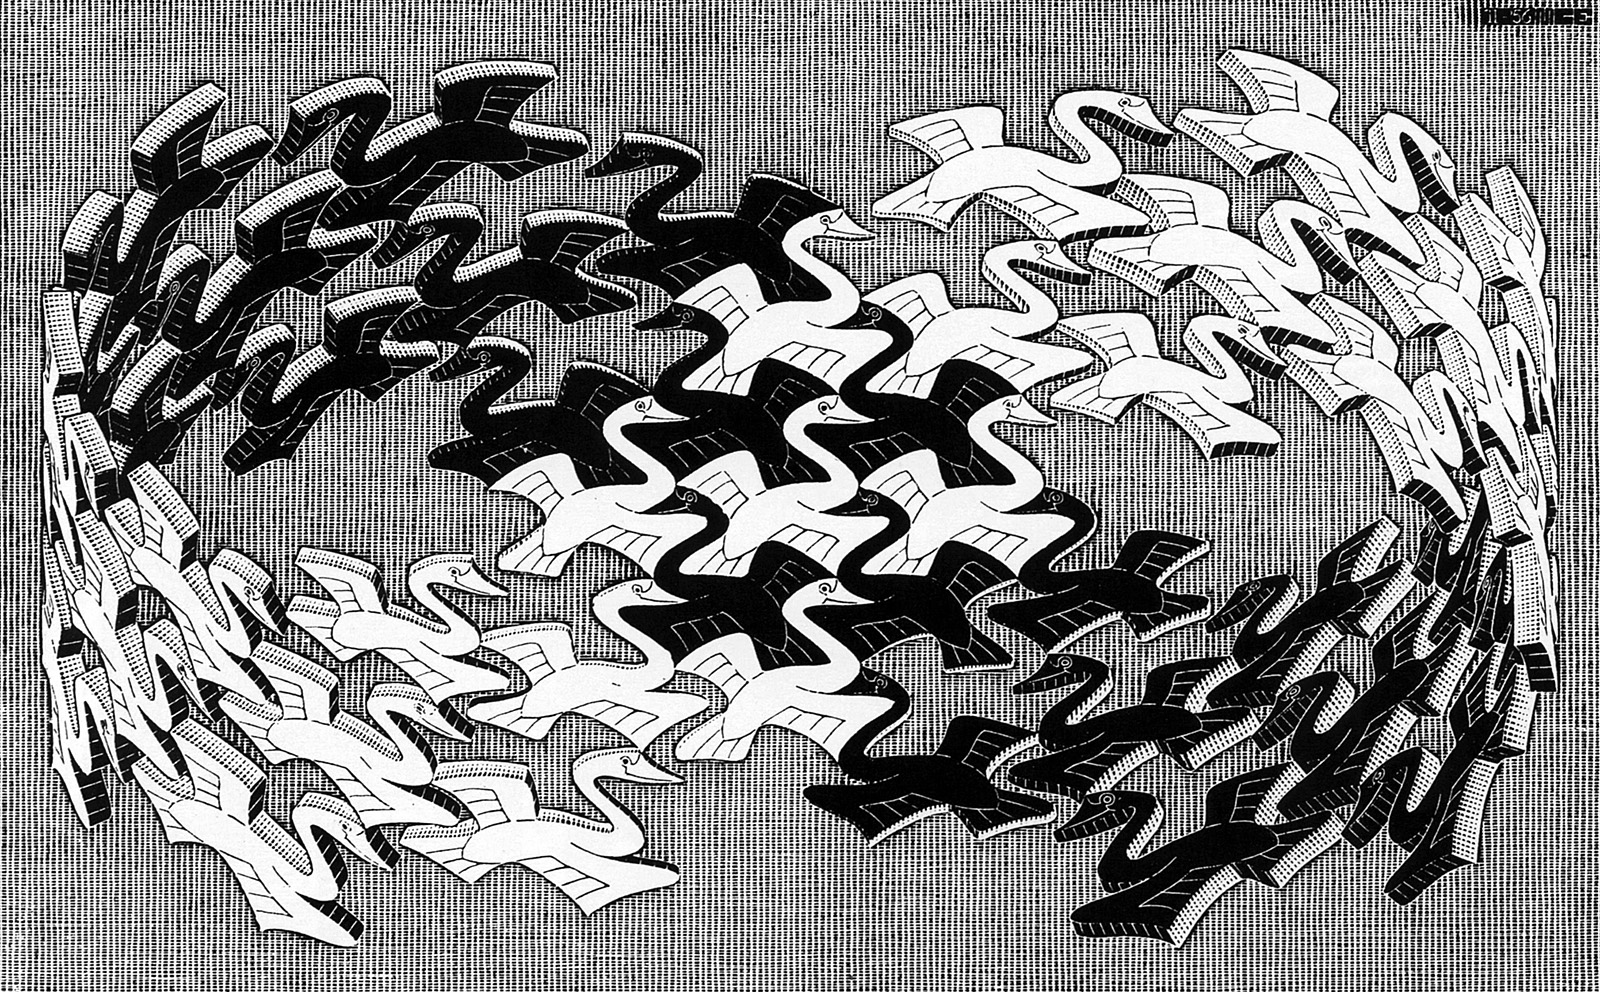
\includegraphics[scale=2]{design_pattern.jpeg}

\vspace{20ex}

Master IT Full Stack Design and Development, a.a. 2022/2023

\end{center}


\newpage

\tableofcontents

%\newpage
%\listoffigures

\newpage

\abstract{}
In questo documento \'e proposto il lavoro relativo alla realizzazione di un \textit{e-shop} di abbigliamento \textit{innovativo}. Una definizione pi\'u precisa di questo aggettivo ha richiesto una fase convergente, legata alla presa di coscienza delle caratteristiche proprie di quelli che sarebbero diventati i nostri \textit{competitors}, nonch\'e una fase divergente, attraverso la quale ci siamo soffermati sulle caratteristiche in linea con quella che iniziava a delinearsi con la nostra definizione di \textit{innovativo} mutuate da domini non appartenenti al mondo dell'\textit{e-shop} e dell'abbigliamento. 
\\
...

\newpage

% capitoli 
\section{Elicitazione dei requisiti}
Questo capitolo raccoglie i requisiti che andranno poi analizzati, modellati e specificati nella fase di \textbf{Analisi dei Requisiti}. 
\\
\\
I problemi comuni da evitare in questa fase iniziale, per uno sviluppo florido del progetto, riferiscono a 3 domini principali:
\begin{enumerate}
	\item \textbf{Scopo}: i requisiti devono riflettere i bisogni del cliente
	\item \textbf{Comprensione}: \'e necessaria una buona comunicazione tra clienti, sviluppatori ed utenti per portare sul pratico i bisogni del cliente, che rifletteranno quelli degli utenti a cui vuole rivolgersi
	\item \textbf{Volatilit\'a}: i requisiti possono cambiare, non essere completi all'inizio dello sviluppo ed evolvere nel tempo; \'e quindi necessario definirli con quanta pi\'u perizia possibile in questa fase del processo
\end{enumerate}

\davide{\textbf{[TODO]} Ampliare la parte sugli strumenti utilizzati per fare la requirement elicitation.}

Si rende quindi necessaria una stretta comunicazione con il cliente, rappresentato dalla Professoressa Bono, per giungere ad un insieme di conoscenze che permetta di superare i problemi esposti poco sopra. \\
La strategia adottata \'e quella dell'\textbf{intervista}, alla quale siamo giunti dopo un \textit{brainstorming} che ci ha visto partecipi in un'iniziale definizione delle caratteristiche che, a nostro parere, dovrebbero appartenere ad un \textit{e-shop innovativo}.
\\
\\
Le nostre riflessioni sono sintetizzate nella sezione successiva. 

\subsection{Analisi di mercato e idee di prodotto} 
In questa fase abbiamo tratteggiato i contorni, ancora sfumati, dell'applicazione. Servono più informazioni possibili per avere una \textbf{visione ampia del mercato} in cui il prodotto richiesto si collocherà, ma anche idee originali a cui ispirarsi, che non devono necessariamente venire dal mondo dell'abbigliamento. Bisogna guardare al di là del {\em main stream}, l'applicazione dovrebbe creare l'effetto wow!
Un'analisi di mercato approfondita ci ha permesso di individuare e confrontare le caratteristiche dei competitors e di pensare a possibili \textbf{soluzioni innovative} non ancora presenti sul mercato da proporre al committente.
\\
\\
...
\\

 
 
\subsection{L'intervista}
...
\\
\\
L'intervista al committente dell'applicazione segue l'iniziale fase di analisi di mercato e di individualizzazione di possibili sviluppi innovativi, la quale è stata essenziale per \textbf{strutturare l'intervista} e raccogliere le idee innovative da proporre al committente. Le informazione raccolte nell'intervista serviranno a definire chiaramente i contorni dell'applicazione e a selezionare i moduli innovativi da sviluppare. L'intervista è stata strutturata nel seguente forma a macro blocchi:

\textbf{Chi:} in questa prima fase conoscitiva abbiamo voluto inquadrare meglio la figura del committente. Abbiamo chiesto:
\begin{itemize}
    \item {\em Descrizione dell'azienda. La sua dimensione e il fatturato? La localizzazione?} Il cliente è l'{\em Atelier Splendor}, una micro azienda di abbigliamento. Possiede una sartoria interna che produce vestiti con il proprio marchio. Attualmente impiega due sarte. Il fatturato non è stato comunicato. L'azienda ha una sola sede nel centro storico di Torino.
    \item {\em Chi sono gli utenti? Target utente finale è basso/medio/alto spandente? giovane/meno giovane, con quali valori e cultura)? Il target futuro deve rimane lo stesso?} Il target di clienti attuale è alto spendente ed è concentrato nella fasci di età tra i 35 e i 60 anni. Il cliente tipo è colto e molto sensibile ai valori della sostenibilità. In futuro l'azienda desidera mantenere il proprio target, estendendolo ulteriormente verso una fascia di età più giovane, ma sempre alto spendente (Quindi max 25 anni, da quando si inizia ad avere uno stipendio).  
    \item {\em Su quale mercato opera attualmente? Su quale mercato punta a operare in futuro?} Attualmente opera sul mercato locale, tipicamente circoscritto alla provincia di Torino. La finalità dell'applicazione del negozio online è anche quella di far varcare i confini ai prodotti dell'{\em Atelier Splendor} e di puntare con la giusta consapevolezza al mercato internazionale.
\end{itemize}

\textbf{Che cosa}: in questa seconda fase sempre conoscitiva abbiamo voluto inquadrare meglio le esigenze del committente. Abbiamo voluto carpire qual'è la sua idea di applicazione finale e le caratteristiche salienti che dovrebbero essere imprescindibili. La raccolta di queste informazioni è stata essenziale per capire il contesto in cui si opera e per selezionare le idee innovative (inizialmente pensate nella fase di analisi di mercato) da proporre al cliente.
\begin{itemize}
    \item {\em Cosa motiva lei e gli stakeholders? Quali sono i vostri valori? In particolare, quali le aspettative in merito al prodotto?} Non vogliamo l’{\em hype} ({\em e.g.} Supreme, vuole la sostanza e la consapevolezza (per se stessi e per l'ambiente). Il cliente dell'{\em Atelier Splendor} sceglie un vestito per dire chi è, non lascia decidere alla massa cosa dovrebbe indossare, chi dovrebbe essere. Questa azienda promuove la cultura dello slow e della consapevolezza. Rifiutando i canoni della GDO, vuole sbarcare sul mercato online seguendo il proprio paradigma.
    \\
    ...
    \item {\em Quali sono gli obiettivi dell’azienda? L’obiettivo principale, gli obiettivi a breve, medio e lungo termine (possibilmente in ordine di importanza)?} L'obiettivo a breve termine è di espandersi attraverso l'apertura di un negozio online. L'obiettivo a medio termine è di farsi conoscere sul mercato.
    \\
    ...
    \item {\em Quali sono i criteri di successo del prodotto? Quali potrebbero essere gli indicatori da monitorare durante il progetto e quale sarebbe un indicatore chiave per stabilire che l'applicazione ha avuto successo?} L'indicatore chiave, tornasole del successo, sarebbe l'impiego di nuovo personale nella sartoria, almeno due nuove sarte.
    \\
    ...
\end{itemize}

\textbf{Quando}: in questa terza fase sempre conoscitiva abbiamo voluto inquadrare meglio le tempistiche relative alla finalizzazione del progetto. Lo scopo di queste domande è di carpire quali/quante idee innovative selezione nella (successiva) fase di brainstorming con il cliente. Il tempo a disposizione determina una selezione che andrà discussa con il cliente e una ripartizione delle idee di valore in moduli ``core", moduli ``pilota" e moduli non presi in considerazione in questa fase.
\begin{itemize}
    \item {\em Quando l'applicazione dovrebbe uscire sul mercato?}
    \\
    ...
\end{itemize}

\textbf{Brainstorming}: in questa fase abbiamo proposto idee al cliente sulla base di quanto raccolto nelle domande precedenti dell'intervista. Le idee proposte sono state avvalorate da una precedente analisi di mercato e dalle conoscenza del nostro esperto di dominio. L'insieme delle idee raccolte è poi stato ridiscusso con il cliente e suddiviso in gruppi, come presente nei risultati.
\\

\subsection{I risultati}

I risultati dell'intervista possono essere suddivisi in tre macro gruppi.
Le idee che per motivi strategici o di tempo non vengono ulteriormente sviluppate sono finite nel gruppo dei moduli attualmente non presi in considerazione, e di seguito non presentati.

La progettazione e lo sviluppo completo dei \textbf{moduli ``core"}, strategici per raggiungere gli obiettivi del cliente e contribuire al tasso di innovazione dell'applicazione. L'investimento del cliente e le forze in gioco del team rendono questi obiettivi realistici e realizzabili.
\\
\piaget{\textbf{[NOTA]} Qui ci sono i moduli da associare a qualche design pattern.}
\begin{itemize}
    \item {\em ``Popup Stores"}: non molti negozi fisici, ma spot stores temporanei, localizzati dove sono concentrati la maggior parte dei clienti. La creazione di una rete di aziende amiche che condividono gli stessi ideali di sostenibilità permette numerosi vantaggi. {\em Atelier Splendor} ospiterà virtualmente i capi di queste aziende nel suo futuro negozio virtuale, queste aziende ospiteranno mostre temporanee dei nostri capi nei loro negozi fisici. La scelta delle città in cui organizzare le mostre verrà suggerita dai dati raccolti.
    \item {\em ``Vestirsi con la realtà aumentata"}: Algoritmo di realtà aumentata stile Ikea che consente di vestirsi virtualmente per provare i vestiti e trovare la propria taglia. Ciò sorride all'ambiente e fa l'occhiolino al consumatore consapevole perché permetterà di ridurre il numero dei resi. Cliente soddisfatto e ambiente pure. 
    \item {\em ``Magazzino Snello"}: rivedere il data model del magazzino da integrare in un data base pinco pallino su cui poggerà la nostra applicazione. Questo consentirà agli impiegati dell'azienda di loggarsi come tali e di monitorare meglio le risorse e i flussi di magazzino, abbattendo i costi generati dalla merce invenduta.
    \item {\em ``Go Circular!"}: sezione dell'applicazione dedicata ai vestiti usati che viene alimentata dai vestiti creati dall'atelier e dati indietro dai clienti in cambio di un vaucher da spendere sui vestiti nuovi confezionati dall'atelier. In questo modo il negozio ospiterà sì brand diversi e sostenibili, ma cerchiamo di favorire l'acquisto di abiti con il nostro brand. Questa politica, che sorride all'ambiente, sorride anche all'espansione della sartoria e all'assunzione di nuovo personale. Inoltre, gli abiti dati indietro spesso necessiteranno una sistemata da parte delle nostre sarte prima di essere caricato online.
    
\end{itemize}

La progettazione e lo sviluppo almeno parziale dei \textbf{moduli ``pilota"}, strategici ai fine del marketing e strategici in futuro, non appena verranno raggiunti gli obiettivi prefissati più importanti (assunzioni di nuove sarte e aumento del numero di clienti). Le condizioni attuali non consentono lo sviluppo completo di questi moduli. Lo sviluppo futuro di questi moduli consentirà una fruttuosa e duratura collaborazione con l'{\em Atelier Splendor}.
\begin{itemize}
    \item {\em ``Algoritmo di consiglio all'acquisto human-driven"}: l'output dell'algoritmo non viene direttamente fornito al cliente, ma è mediato dall'essere umano, nello specifico un esperto di moda, che spiega il perché di questo consiglio di acquisto.
    \item {\em ``Marketing"}: Nell'ambito del marketing, prodotti mirati saranno associati a un link di un contento Tiktok di un influencer che starà indossando quel vestito. Questo per ampliare il target verso una fascia più giovane.
    \item {\em ``Sartoria dedicata e confezionamento su misura"}: la sartoria interna potrà essere ulteriormente allargata introducendo due nuovi servizi al cliente. Primo, i vestiti che necessiteranno di manutenzione (orli, pence, sostituzione cerniere, rattoppi, ...) potranno essere spediti alla sede centrale per essere aggiustati. Due, la sartoria offrirà la possibilità di avere abiti confezionati su misura.
\end{itemize}

\davide{\textbf{[TODO]} Rivedere e aggiungere informazioni nelle risposte. Scegliere bene i nomi dei moduli, che potrebbero poi essere utilizzati nello sviluppo dei design pattern.}

\section{Analisi dei requisiti}

In questa sezione riportiamo i requisiti che la nostra applicazione dovrà rispettare e seguire nello sviluppo...

\andrea{\textbf{TO DO} Accorpare sezione di attori e casi d'uso, visto che la tassonomia proposta e' in funzione del contesto.}

\subsection{Gli attori e i loro obiettivi}

\begin{itemize}
    \item Gli \textbf{attori principali} sono quelli che utilizzano direttamente l’applicazione per uno specifico use case (sono i fruitori dell’app, e.g. un cliente, un impiegato).
    \item Gli \textbf{attori secondari} sono sistemi esterni (tipicamente software) che integriamo all’interno dell’app (sono API che inseriamo per implementare il tutto e su cui non abbiamo controllo).
    \item Gli \textbf{attori fuori scena} sono entità che non usano direttamente l’app, ma che ne possono trarre benefici o ci danno dei vincoli da rispettare (l’università è l’attore fuori scena che beneficia di Moodle, la legge con il GDPR).
\end{itemize}


\davide{\textbf{[TODO]} Elencare gli attori (principali, secondari, fuori scena) e i loro obiettivi.}

\subsection{I casi d'uso}
\label{subsec:UC}

L'{\em UC diagram} è una “interfaccia” astratta della nostra applicazione, che descrive un possibile {\em caso d'uso}, ossia un possibile scenario di utilizzo dell'applicazione, figura \ref{fig:UC_diagram}.


\andrea{\textbf{TO DO} terzo UC3 = POP-UP STORE = aggiorna sezione sotto}


Casi d'uso ipotizzati a lezione:
\begin{itemize}
    \item Voglio comprare un vestito online,
    \item Voglio accedere al magazzino snello,
    \item Pop-Up store  
\end{itemize}

Attori e ruoli:
\begin{itemize}
	\item UC1
		\begin{itemize}
		\item attore principale: cliente - dipendente  
		\item attore secondario: metodi di pagamento 
		\item fuori scena: corriere (pacchi, beneficia del mio indotto)
		\end{itemize}
	\item UC2
		\begin{itemize}
		\item attore principale: sarto (fa abito e gestisce) - utente/avatar 
		\item attore secondario: algoritmo/gestionale
		\item fuori scena: fornitori materie prime/tessuto 
		\end{itemize}
	\item UC3
		\begin{itemize}
		\item attore principale: cliente - dipendente/cliente 
		\item attore secondario: database collegato a software tramite API per andare a salvare i vari utenti che lasciano email e autorizzazioni per la newsletter 
		\item fuori scena: GDPR - software per crittografare 
		\end{itemize}
\end{itemize}

I {\em requisiti funzionali} riguardano ciò che il sistema fa e sono i moduli da implementare o integrare per lo sviluppo dell’applicazione.
I {\em requisiti non funzionali} riguardano com’è fatto il sistema. Esempi di requisiti non funzionali sono i tool che scelgo, il linguaggio di programmazione che uso, data base che scelgo, ...
\\
\\
Requisiti:
\begin{itemize}
	\item UC1
		\begin{itemize}
		\item funzionali: voglio permettere all'utente di accedere al mio sito web e alla mia applicazione, visualizzare l'elenco degli articoli a mia disposizione, fargli scegliere quelli che pi\'u lo aggradano, inserirli nel carrello, pagare e completare l'ordine. Voglio permettere al dipendente di visualizzare gli ordini 
		\item non funzionali: tools Java (pattern decorator + strategy), html+javascript+css (front-end), Oracle. 
		\end{itemize}
	\item UC2
		\begin{itemize}
		\item funzionali: voglio permettere all'utente di gestirsi (eventualmente) l'avatar, tramite cui provera' le diverse combinazioni di capi. I dati immagazzinati serviranno al sarto per una gestione pi\'u lean del magazzino (vedi anche ordini con i fornitori di materie prime)
		\item non funzionali: Oracle, Java (pattern Composite), three-js (libreria js sul browser per realt\'a aumentata)/ webGL (grafica 3D)
		\end{itemize}
	\item UC3
		\begin{itemize}
		\item funzionali: voglio permettere ai miei "iscritti" di ricevere info riguardanti i prossimi eventi pop-up store nella zona geografica di competenza 
		\item non funzionali: Oracle, Java (pattern Observer), client mail, API di geolocalizzazione
		\end{itemize}
\end{itemize}


\vspace{1em}
\begin{figure}[ht]
  \centering
   \makebox[\textwidth][c]{\includesvg[width= 1.1\linewidth]{UC_diagram.svg}}
  \caption{\small Esempio di UC diagram relativo all'applicazione del negozio online. All'interno delle {\em system boundaries} sono posizionati i casi d'uso esaminati in questa sezione. Gli attori principali (azzurro), quelli secondari (verde) e quelli fuori scena (giallo) sono rappresentati dalle figure al di fuori del {\em system} e sono collegati ai relativi casi d'uso. Una più approfondita analisi del diagramma è presentata in sezione \ref{subsec:UC}}
  \label{fig:UC_diagram}
\end{figure}


\subsection{Glossario degli attori}

\andrea{\texbf{TODO} Termini di informatichese per il cliente che non ne sa nulla. Prendi termini "difficili" di sezione precedente e definiscili.}

\davide{\textbf{[TODO]} Elaborare il contenuto e scrivere questa sezione.}

...


\section{Il documento di vision}

\edoardo{\textbf{TODO} Elabora}

\davide{\textbf{[TODO]} Elaborare il contenuto e scrivere questa sezione.}

...


\section{Design Patterns utilizzati}

Un {\em pattern} è una soluzione generale ad un problema ricorrente, che va opportunamente adattato al problema in esame. Un Pattern può essere riassunto in: problema, soluzione, pro e contro della soluzione ed esempi d’uso. I Design pattern visti a lezione sono i \textbf{GoF Design Pattern} e permettono di sfruttare al massimo le caratteristiche object oriented di Java. Essi costituiscono di fatto una mappa per scrivere codice Java.

In questa sezione riportiamo sottoforma di micro-prototipi le implementazioni dei design pattern applicati ai casi d'uso della nostra applicazione.

\begin{itemize}
    \item Con riferimento al caso d'uso dell'acquisto abito sull'applicazione. Un impiegato dell'atelier può anche essere un cliente e utilizzare l'applicazione con due scopi differenti.
    Abbiamo quindi pensato di modellare la figura dell' impiegato-cliente tramite due pattern alternativi: il \textbf{pattern Decorator} e il \textbf{pattern Strategy}. Ciò ci ha permesso di confrontare e discutere i vantaggi/svantaggi dei due patterns.
    \item Riferimento al caso d'uso dell'accesso al magazzino snello, possiamo ricollegarci al modulo sull'approccio human-driven per implementare il \textbf{pattern Composite}. Lato tecnico usiamo il pattern composite. Lato umano, i sottoinsiemi generati dal composite verranno filtrati dall'umano esperto.
    Alternativamente, il pattern composite potrebbe essere applicato semplicemente al caso d'uso dell'accedere al magazzino snello con riferimento al modulo del {\em magazzino snello}.
\end{itemize}


\andrea{\textbf{[NOTA]} Obbligatorio il design pattern {\em Composite} con almeno tre livelli che restituisca, e.g. le componenti di abbigliamento che formano l'outfit. Più siamo fantasiosi nel trovare un'applicazione tra le nostre idee, meglio verrà valutato.}

\davide{\textbf{[TODO]} Aggiungere la bibliografia con i testi e documenti riportati su moodle.}

\davide{Materiale da citare: \cite{gof_riferimento}, \cite{up-riferimento}, \cite{uml_riferimento}, \cite{elicitation_tools}, \cite{gof_sunt}, \cite{github}.}


\subsection{Pattern Decorator}

Il {\em pattern Decorator} permette di aggiungere dinamicamente responsabilità addizionali ad un oggetto. In questo modo si possono estendere le funzionalità di oggetti particolari senza coinvolgere intere classi \cite{gof_sunt}.
Con riferimento al caso d'uso dell'acquisto di un abito sull'applicazione, si pensi ad un modello di oggetti che rappresenti gli impiegati dell'atelier Splendor. Un impiegato può diventare un cliente interessato a comprare un abito sulla piattaforma. Nasce così l'esigenza di modellare la figura dell'\textbf{cliente-dipendente}, il quale in aggiunta alle operazioni definite per gli impiegati, definisce anche quelle relative ai clienti.

Il pattern suggerisce la creazione di {\em wrapper classes} (Decorator) che racchiudono gli oggetti ai quali si vuole aggiungere le nuove responsabilità. Questi ultimi oggetti, insieme ai Decorator devono implementare una interfaccia comune, in modo che l’applicazione possa continuare ad interagire con gli oggetti decorati \cite{gof_sunt}.
Per una stessa interfaccia possono esserci più Decorator, ma in questo caso ne considereremo solo uno.

\davide{\textbf{[TODO]} Il codice del decorator va completamente rivisto e ampliato.}

\lstinputlisting[label={list:esempio}, caption={\small ClienteDipendente.java -- Implementazione del pattern Decorator nel caso d'uso dell'acquisto online.}]
{code/ClienteDipendente.java}


\subsection{Pattern Strategy}

Il {\em pattern Strategy} serve a definire una famiglia di algoritmi simili tra loro e dunque \textbf{intercambiabili}. In particolare, è tipica della situazione in cui vogliamo isolare l’algoritmo che svolge un certo compito, per farlo variare in modo indipendente dal resto dell’implementazione della classe.

Questo pattern suggerisce l’incapsulamento della logica di ogni
particolare algoritmo, in apposite classi, dette {\em ConcreteStrategy}, le quali implementano l’interfaccia che consente agli oggetti di interagire con loro. Questa interfaccia deve fornire un accesso efficiente ai dati del Context, richiesti da ogni ConcreteStrategy, e viceversa \cite{gof_sunt}.


\subsection{Pattern Composite}

\davide{\textbf{[TODO]} Sviluppare il microprototipo del pattern Composite per il caso studio del magazzino snello.}

\subsection{Pattern Observer}

\andrea{\textbf{TODO} A codice ultimato, scrivi sezione}


\newpage

%Prints the bibliography
\printbibliography


\end{document}